%=========|CABECALHO|=========>
\thispagestyle{empty}
\center
\begin{minipage}[!]{\linewidth}
	\begin{minipage}[!]{.19\linewidth}
		
\includegraphics[width=\textwidth]{img/Marca Joinville Vertical RGB-01.jpg}				
	\end{minipage}
	\begin{minipage}[!]{.8\linewidth}
		\center
		\textsf{
			\large{
				\instituicao \\ \vspace{0.1cm}
				\centro \\ \vspace{0.17cm}
				\departamento
				%\disciplina
			}	
		}		
	\end{minipage}
	\center
	\rule{\textwidth}{1pt}	
	\textsc{\autor} \\
	\today \\ 
	\rule{\textwidth}{1pt}	
\end{minipage}
%\vspace{1cm}
\begin{center}
   \textbf{\titulo}\\  
   \rule{.3\textwidth}{0.1pt}
\end{center}
\renewcommand{\thesection}{\Roman{section}}
%=========|END-CABECALHO|=====>


%============| INÍCIO |=======================================>
%--------------| Q01 |---------------------------------------->
\begin{prob}
	Mostre que:
	\begin{enumerate}[label=\alph *)]
		\item $1\textnormal{ ano-luz}=9,46\times 10^{12}km$
		\item $1\textnormal{ parsec}=3,26\textnormal{ anos-luz, i.e. }3,08\times10^{13}km$
	\end{enumerate}	
\end{prob}


\begin{sol}
	\textcolor{teal} {
		Considerando $v_l=299.792.458m/s$ para a velocidade da luz e $t=31.557.600s$ para o período de um ano
		\begin{enumerate}[label=\alph *)]
			\item $1\textnormal{ ano-luz}=(v_l)t=(3,0\times 10^{8}m/s)(3,1\times 10^{7}s)=9,46\times 10^{15}m=9,46\times 10^{12}km$
			\item 1 parsec $=3,26\times(9,46\times 10^{12}km)=3,08\times10^{13}km.$
		\end{enumerate}
	}	
\end{sol}

%--------------| Q02 |---------------------------------------->
\begin{prob}
	Quando o Sol se põe, decorrem aproximadamente 2 minutos entre o instante em que o disco solar encosta no horizonte e sua ocultação completa. A partir deste dado, estime o diâmetro angular aparente do Sol visto da Terra, em graus.
\end{prob}

\begin{sol}
	\textcolor {teal} {
		Assumindo um dia em que o sol demora 12 horas entre o nascer e o ocaso temos que
		\begin{align}
			\frac{\theta_{sol}}{180^{\circ}}&=\frac{2min}{720min}\quad \therefore\quad\theta_{sol}=0,5^{\circ}			
		\end{align}
	}
\end{sol}

%--------------| Q03 |---------------------------------------->
\begin{prob}
	No dia do solstício de verão (o mais longo do ano), na cidade de Siena, ao meio dia, os raios solares eram exatamente verticais. Neste dia e hora, Eratóstenes mediu a sombra projetada por uma
	estaca vertical na cidade de Alexandria e descobriu que ela tinha um oitavo da altura da estaca. Além disso, a distância entre as duas cidades já era conhecida como 5000 estádios (1 estádio aproximadamente 157 metros). Com estes dados, calcule o raio da Terra.
\end{prob}

\begin{sol}
	\textcolor{teal} {
		Sabe-se que o comprimento $C$ de uma circunferência de raio $R$ é dado por:
		\begin{align}
			C&=2\pi R
			\label{eq:comprimento-circ}
		\end{align}
		Da eq. \eqref{eq:comprimento-circ} é fácil de ver que se soubermos $C$, então $R$ é imediato. Outro ponto a se considerar é o comprimento do arco de um setor da mesma circunferência dado por
		\begin{align}
			c&=\alpha R
			\label{eq:comprimento-setor}
		\end{align}
		estas grandezas são proporcionais de modo que
		\begin{align}
			\frac{C}{c}&=\frac{2\pi R}{\alpha R}
		\end{align}
		logo
		\begin{align}
			C&=c\left(\frac{2\pi}{\alpha}\right)
		\end{align}
		no caso:
		\begin{itemize}
			\item C é o comprimento da circunferência terrestre;
			\item c é o comprimento do arco de circuferência, que vai de Siena a Alexandria;
			\item $\alpha$ é o ângulo entre as duas cidades medido a partir do centro da terra, essencialmente o mesmo ângulo que o raio de sol incide na estaca em Alexndria. 
		\end{itemize}
		Para determinar $\alpha$ (em Alexandria), basta fazer
		\begin{align}
			\tan \alpha&=\frac{h/8}{h}=\frac{1}{8} \nonumber \\
			\alpha&=\arctan\left(\frac{1}{8}\right) \nonumber \\
			\alpha&=7,13^{\circ}
		\end{align}
		Assim
		\begin{align}
			C=5000\times 157m\left(\frac{360^{\circ}}{7,13^{\circ}}\right)=3,96\times 10^{7}m
		\end{align}
		e por fim
		\begin{align}
			R=\frac{C}{2\pi}=6,30\times 10^{6}m
		\end{align}
	}
\end{sol}
%--------------| Q04 |---------------------------------------->
\begin{prob}
	O diâmetro angular da Lua pode ser determinado com o auxílio de uma régua. Estique um braço com a régua na mão e alinhe a extremidade superior da régua com a extremidade superior da Lua. Coloque o polegar no ponto da régua que coincide com a extremidade inferior da Lua.
	\begin{enumerate}[label=\alph *)]
		\item Em termos de $d$ e $x$, quanto vale o diâmetro da Lua? Resultados típicos da razão $x/d$ giram em torno de $1/110$.
		\item Como poderímaos utilizar as informações acima para calcular a razão entre a distância da Lua e seu diâmetro.
	\end{enumerate}
\end{prob}
%--------------| Q05 |---------------------------------------->
\begin{prob}
	No século III A.C, o astrônomo Aristarco de Samos estimou a razão $d_{S}/d_{L}$ entre a distância $d_{S}$ da Terra ao Sol e distância $d_{L}$ da Terra à Lua medindo o ângulo $\theta$ entre as retas Terra-Sol e Terra-Lua. O valor obtido foi $\theta=87^{\circ}$.
	\begin{enumerate}[label=\alph *)]
		\item Encontre a estimativa de Aristarco para $d_{S}/d_{L}$.
		\item Com base nos valores atualmente conhecidos, $d_{S}/d_{L}\sim 389$. Determine o valor atual de $\theta$ e argumente porque o método de Aristarco não produz um bom resultado.
	\end{enumerate}
\end{prob}
%--------------| Q06 |---------------------------------------->
\begin{prob}
	Deduza a forma que a latitude de um observador se relaciona com a altura do polo elevado.
\end{prob}
\begin{sol}
	\textcolor{teal} {
		Os autores \cite{ASTRN&ASTRFIS:2004} definem, a latitude geográfica como sendo o ângulo $\phi$ medido ao longo do meridiano local, com origem no equador $E$ e extremidade no zênite local $z_{O}$.\\				
		A figura \eqref{fig:angulos-coordGeo}, representa um observador localizado no ponto $O$ do planeta (circunferência), e de latitude $\phi$. O zênite do observador está representado pelo segmento de reta $z_{O}$ e o seu horizonte pelo segmento de reta $h_O$. Um dos pólos do planeta é representado pela segmento de reta $P$, perpendicular ao equador $E$. Por fim, obtêm-se a reta auxiliar $g$ transladando $h_O$ paralelarmente até o centro $C$ da circunferência. Deseja-se demostrar que o ângulo $\beta$, denominado altura do pólo elevado $h_P$, é essencialmente igual a latitude local $\phi$ do observador.	
		\begin{figure}[!ht]
			\centering
			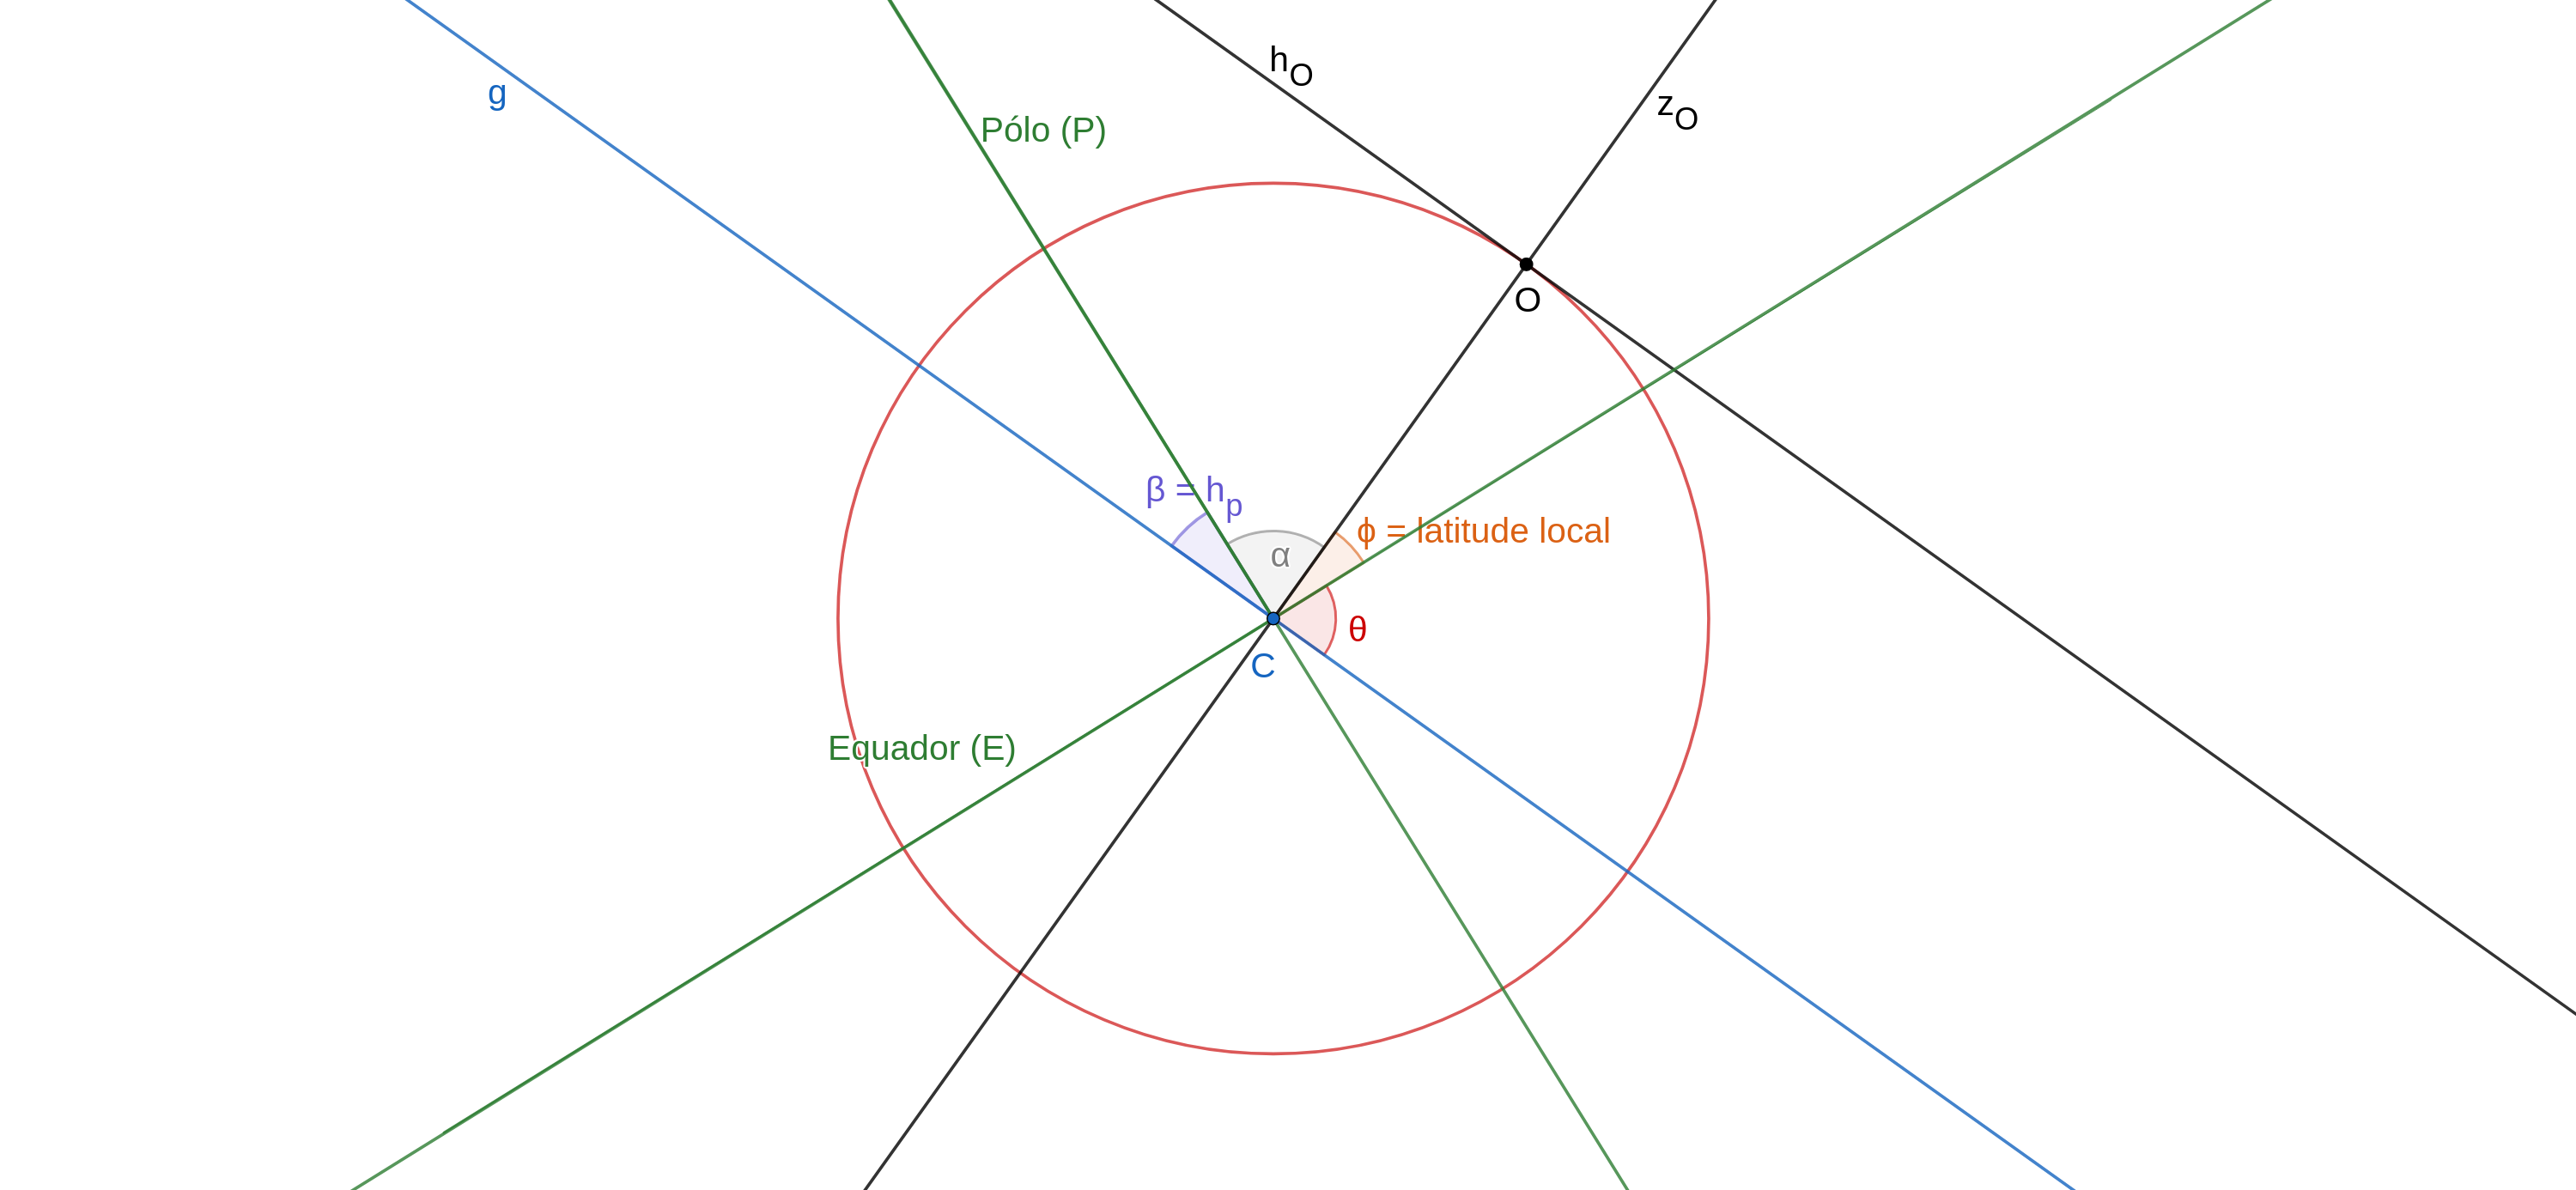
\includegraphics[width=\textwidth]{fig/geogebra-export.png}
			\caption{Diagrama dos ângulos entre as diversas coordenadas geográficas}
			\label{fig:angulos-coordGeo}
		\end{figure}
	}
	
	\textcolor{teal} {
		Nota-se de imediato que
		\begin{align}
			\pi&=\beta+\alpha+\phi+\theta
		\end{align}
		\begin{align}
			\frac{\pi}{2}&=\alpha+\phi
		\end{align}
		\begin{align}
			\frac{\pi}{2}&=\phi+\theta
		\end{align}
		Resolvendo o sistema de equações tem-se
		\begin{align}
			\beta+\alpha+\phi+\theta-\alpha-\phi-\phi-\theta&=\pi-\frac{\pi}{2}-\frac{\pi}{2} \nonumber \\
			\beta-\phi&=0 \nonumber \\
			\beta&=\phi
		\end{align}
	}
	
\end{sol}
%--------------| Q07 |---------------------------------------->
\begin{prob}
	Verifica-se que, em um certo lugar do hemisfério sul, os círculos diurnos das estrelas fazem um
	ângulo de $50^{\circ}$ com o horizonte.
	\begin{enumerate}[label=\alph *)]
		\item Qual a latitude do lugar?
		\item Qual o pólo elevado (norte ou sul) e qual a sua altura (elevação acima do horizonte)?
	\end{enumerate}
\end{prob}

\begin{sol}
	\textcolor{teal} {
		Cículos diurnos são sempre paralelos ao equador celeste, neste caso o horizonte encontra-se a um ângulo de $50^{\circ}$ com o equador e portanto:
		\begin{enumerate}[label=\alph *)]
			\item A latitude do local pode ser calculada pelo ângulo de declinação, sendo $\delta=90^{\circ}-50^{\circ}$ ou seja $\delta=\phi=40^{\circ}$
			\item Sul é o pólo elevado e por definição $h_p=\phi=40^{\circ}$
		\end{enumerate}
	}
\end{sol}
%--------------| Q08 |---------------------------------------->
\begin{prob}
	Para um observador no equador da Terra:
	\begin{enumerate}[label=\alph *)]
		\item Qual a altura do pólo celeste norte?
		\item E do pólo celeste sul?
		\item Como é o movimento das estrelas nesse lugar, com relação ao horizonte?
		\item Existem estrelas circumpolares nesse lugar?
	\end{enumerate}
\end{prob}

\begin{sol}
	\textcolor{teal} {
		\begin{enumerate}[label=\alph *)]
			\item $0^{\circ}$
			\item $0^{\circ}$
			\item O movimento das estrelas se da a um ângulo de $90^{\circ}$ do horizonte
			\item Não há estrelas circumpolares
		\end{enumerate}
	}
\end{sol}
%--------------| Q09 |---------------------------------------->
\begin{prob}
	Desenhe um circulo representando a esfera celeste para um observador localizado em uma lugar
	de latitude $20^{\circ}N$. Nesse círculo marque:
	\begin{enumerate}[label=\alph *)]
		\item A localização do zênite
		\item A localização do pólo elevado, e o ângulo que ele faz com o horizonte
		\item O plano do equador
		\item O plano do horizonte, com os pontos cardeais $N,S,L,O$
		\item A calota das estrelas circumpolares visíveis
		\item O círculo diurno de uma estrela de declinação $\delta=+40^{\circ}$
	\end{enumerate}
\end{prob}
%--------------| Q10 |---------------------------------------->
\newpage
\begin{prob}
	Entre as estrelas da tabela \eqref{tab:tabela_ascencao-declinacao}, escolha:
	\begin{enumerate}[label=\alph *)]
		\item As que pertencem ao hemisfério sul celeste
		\item As que nunca podem ser vista em Oslo $(latitude=59^{\circ}N)$
		\item A(s) que é(são) circumpolar(es) em Porto Alegre $(latitude=30^{\circ}S)$
		\item A que faz sua passagem meridiana mais próxima do zênite em Porto Alegre
		\item As que estão na faixa do zodíaco
	\end{enumerate}
	\begin{table}[!ht]
		\centering
		\caption{Medidas de ascensão reta e ângulo de declinação de algumas constelações}
		\label{tab:tabela_ascencao-declinacao}
		\begin{tabular}{r|cc|c|}
		\cline{2-4}
		\multicolumn{1}{l|}{}                  & \multicolumn{2}{c|}{\textbf{Ascensão reta $(\alpha)$}} & \textbf{Declinação $(\delta)$} \\ \hline
		\multicolumn{1}{|c|}{\textbf{Estrela}} & \multicolumn{1}{c|}{hora $(h)$}    & min $(\prime)$    & graus $(\circ)$                \\ \hline
		\multicolumn{1}{|r|}{Sírius ($\alpha$-Cão Maior)}  & \multicolumn{1}{c|}{6}  & 45 & -17   \\ \hline
		\multicolumn{1}{|r|}{Canopus ($\alpha$-Carina)}     & \multicolumn{1}{c|}{6}  & 54 & -53   \\ \hline
		\multicolumn{1}{|r|}{Vega ($\alpha$-Lira)}         & \multicolumn{1}{c|}{18} & 37 & +39   \\ \hline
		\multicolumn{1}{|r|}{Antares ($\alpha$-Escorpião)} & \multicolumn{1}{c|}{16} & 29 & -26,5 \\ \hline
		\multicolumn{1}{|r|}{Betelgeuse ($\alpha$-Orion)}  & \multicolumn{1}{c|}{5}  & 55 & +7    \\ \hline
		\multicolumn{1}{|r|}{Deneb ($\alpha$-Cisne)}        & \multicolumn{1}{c|}{20} & 41 & +45    \\ \hline
		\multicolumn{1}{|r|}{Arcturus ($\alpha$-Bootis)}   & \multicolumn{1}{c|}{14} & 15 & +19   \\ \hline
		\multicolumn{1}{|r|}{Acrux ($\alpha$-Crucis)}      & \multicolumn{1}{c|}{12} & 26 & -63   \\ \hline
		\multicolumn{1}{|r|}{Spica ($\alpha$-Virgem)}      & \multicolumn{1}{c|}{13} & 25 & -11   \\ \hline
		\multicolumn{1}{|r|}{Rigelkent ($\alpha$-Centauri)} & \multicolumn{1}{c|}{14} & 39 & -61   \\ \hline
		\multicolumn{1}{|r|}{Rigel ($\beta$-Orionis)}      & \multicolumn{1}{c|}{5}  & 14 & -8    \\ \hline
		\end{tabular}
		\end{table}
\end{prob}
\newpage
%--------------| Q11 |---------------------------------------->
\begin{prob}
	Mostre que um dia sideral é aproximadamente $4min$ mais curto que o dia solar.
\end{prob}
%--------------| Q12 |---------------------------------------->
\begin{prob}
	A latitude em Montreal é $48^{\circ}N$
	\begin{enumerate}[label=\alph *)]
		\item Sabendo que a obliquidade da eclíptica é $23,5^{\circ}$, qual a altura máxima do Sol, no verão, em Montreal Faça um desenho explicativo
		\item Se em Porto Alegre a máxima altura do Sol, no verão, é $83,5^{\circ}$, calcule a razão entre a insolação recebida em Montreal, no verão, com a insolação recebida em Porto Alegre, no	verão.
		\item Se a obliquidade da eclíptica fosse $33^{\circ}$, qual seria o efeito nas estações, comparado com a obliquidade real, de $23,5^{\circ}$,
		\begin{enumerate}[label=\alph{enumi}.\roman{enumii})]
			\item em Montreal
			\item em uma cidade localizada no equador
		\end{enumerate}				
	\end{enumerate}
\end{prob}
%--------------| Q13 |---------------------------------------->
\begin{prob}
	Uma astro realiza, durante o período de um dia, duas passagens meridianas. Considere uma
	estrela que faz uma passagem meridiana a uma altura de $85^{\circ}$, ao sul do zênite, e uma segunda
	passagem a uma altura de $45^{\circ}$, ao norte do zênite. Calcule a declinação da estrela e a latitude do
	observador.
\end{prob}
%--------------| Q14 |---------------------------------------->
\begin{prob}
	Considere a culminação superior de um astro. Deduza uma relação para a distância zenital em
	termos da declinação dos astro e da latitude do observador. Note que a relação deve ser ligeiramente
	diferente para culminação ao norte do zênite ou ao sul do zênite.
\end{prob}
%--------------| Q15 |---------------------------------------->
\begin{prob}
	Encontre uma relação entre o módulo da latitude do observador e o módulo da declinação de
	uma estrela para que esta seja circumpolar.
\end{prob}
%--------------| Q16 |---------------------------------------->
\begin{prob}
	A longitude de Porto Alegre é de, aproximadamente, $-51^{\circ}$. Sabendo que Porto Alegre está no
	fuso $-3h$, em quanto tempo a sua hora real está atrasada ou adiantada em relação à Hora Legal (hora
	do fuso).
\end{prob}